\documentclass[a4paper, 12pt]{article} %mémoire en A4, police 12

%--------------------------------------------------------------------------------------- Les packages utilisés                                                                            %----------------------------------------------------------------------------------------
\usepackage{xcolor} %pour les couleurs
\usepackage[utf8]{inputenc} %pour l'écriture
\usepackage[french]{babel} %pour avoir les textes automatiques en français
\usepackage{amsmath} %pour ecrire des maths
\usepackage{setspace}
\setstretch{0.7}
\usepackage{amsfonts} %pour ecrire des maths
\usepackage{amssymb} %définit des symboles mathématiques
\usepackage{graphicx} %pour les graphes
\graphicspath{ {./Images/}}
\usepackage{mathtools}
\usepackage[left=2cm,right=2cm,top=2.5cm,bottom=2.5cm]{geometry} %formatage du document
\usepackage{url} %pour mettre des urls
\usepackage{fancyhdr} %pour le formatage des pages
\usepackage{tcolorbox}
\usepackage{tikz}

\title{\textbf{Tutoriel de séries temporelles linéaires}}
\author{Thomas Dujardin, Bastian Dupoirieux}
\date{Avril - Mai 2022}

%---------------------------------------------------------------------------------Formatage des pages

\pagestyle{fancy}
\fancyhf{}
\lhead{Séries temporelles linéaires}
\rhead{ENSAE Paris}
\cfoot{\thepage}
%---------------------------------------------------------------------------------


\begin{document}



\maketitle


\Large{\textbf{Partie I : Les données}}
\begin{tcolorbox}
{\small
1. Que représente la série choisie ? (secteur, périmètre, traitements éventuels, transformation logarithmique, etc.)}
\end{tcolorbox}
{\normalsize
{La série choisie représente l'indice CVS-CJO (Corrigé des Variables Saisonnières - Corrigé des Jours Ouvrés) en base 100 en 2015 (donc de moyenne 100 en 2015) de la production aéronautique et spatiale entre janvier 1990 et janvier 2020.}}

\begin{figure}[h]
    \centering
    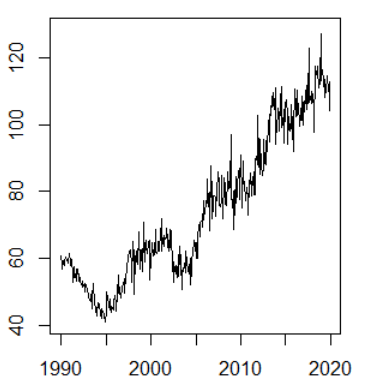
\includegraphics[scale =0.7]{serie_ae.png}
    \caption{Série initiale}
\end{figure}

\begin{tcolorbox}
{\small
2. Transformer si besoin la série pour la rendre stationnaire (différentiation, suppression de la tendance
déterministe, etc.). Justifier soigneusement vos choix.}
\end{tcolorbox}
{\normalsize
{La figure 1 ci-dessus montre une tendance. Une régression linéaire de l'indice sur la date montre que les coefficients correspondant à une tendance (date et constante) sont significatifs (p-value de la nullité jointe inférieure à 0.05). }}
\begin{table}[h]
    \centering
    \fbox{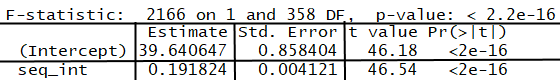
\includegraphics[scale =0.7]{lm_non_diff_aero.png}}
    \caption{Régression linéaire de l'indice sur la date}
\end{table}
{\normalsize
{Nous allons donc effectuer un test de la racine unitaire avec constante et tendance. Il faut d'abord vérifier la non-autocorrélation des résidus de la régression linéaire ci-dessus. Un premier ADF sans lags avec les 24 derniers résidus (donc sur deux ans) est rejeté à tous les ordres. Il faut alors inclure au minimum 7 lags afin de supprimer l'autocorrélation des résidus. \newline Ce test ADF à 7 lags donne une p-value pour la tendance de \textbf{0.1595} $>$ 0.05 : on ne peut pas rejeter la non-stationnarité au seuil de 5 (pourcent). Il est donc nécessaire de différencier au moins une fois la série.}}
\\ \\{\normalsize
{Testons la présence d'une tendance dans la série différenciée :}}
\begin{table}[h]
    \centering
    \fbox{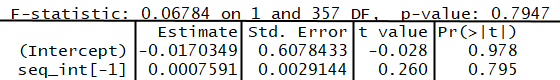
\includegraphics[scale =0.7]{lm_diff_aero.png}}
    \caption{Régression linéaire de l'indice différencié sur la date}
\end{table}
{\normalsize
{\\Nous déterminons ensuite qu'il faut 6 lags pour supprimer l'autocorrélation des résidus de cette seconde régression linéaire, et qu'un test ADF à 6 lags donne une p-value de moins de \textbf{0.01}, donc un rejet de l'hypothèse de racine unitaire à tous les niveaux, et donc la stationnarité de la série différenciée.}}
\begin{tcolorbox}
{\small
3. Représenter graphiquement la série choisie avant et après transformation.
}
\end{tcolorbox}
\begin{figure}[h]
    \centering
    \fbox{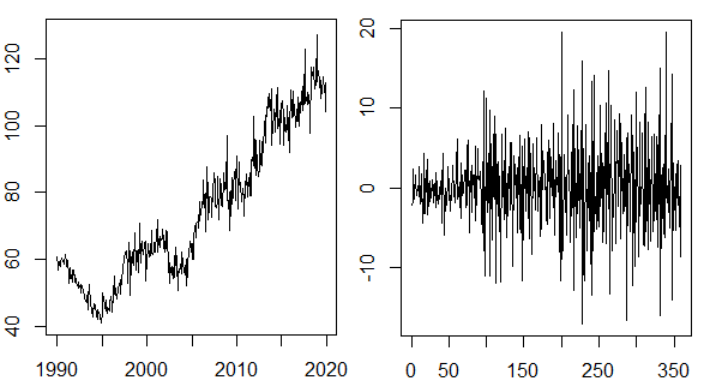
\includegraphics[scale =0.5]{aero_diff_non_diff.png}}
    \caption{Série brute (gauche) et série différenciée (droite)}
\end{figure}
\Large{\textbf{Partie II : Modèles ARMA}}
\begin{tcolorbox}
{\small
4. Choisir, en le justifiant, un modèle ARMA(p,q) pour votre série corrigée X$_t$. Estimer les paramètres
du modèle et vérifier sa validité.
}
\end{tcolorbox}
{\normalsize
{On détermine les fonctions d'autocorrélations et d'autocorrélations partielles :
}}
\begin{figure}[h]
    \centering
    \fbox{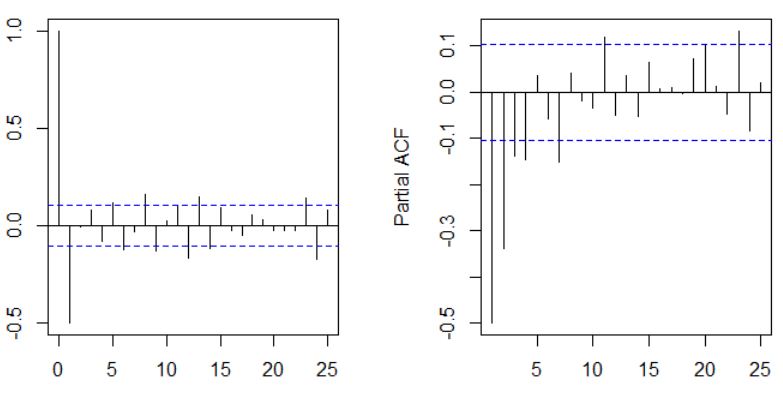
\includegraphics[scale =0.4]{aero_acf_pacf.png}}
    \caption{ACF, PACF de la série différenciée}
\end{figure}
\newpage
\normalsize{
{On observe des valeurs significatives jusqu'à des ordres élevés, mais on ne retiendra que les pics $p_{max} = 11$ (d'après la PACF) et $q_{max} = 14$ (d'après l'ACF).\\
On détermine alors les AICs et BICs des $ARIMA(p, 1, q)$ où $p \leqslant p_{max}$ et $q \leqslant q_{max}$. On obtient que $ARIMA(0, 1, 1)$ (donc MA(1)) et $ARIMA(2, 1, 2)$ minimisent respectivement BIC et AIC.\\ \\On va maintenant tester les autocorrélations des résidus de ces deux modèles, et tester leur ajustement :
}}
\begin{figure}[h]
    \centering
    \fbox{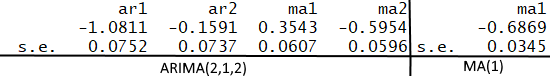
\includegraphics[scale =0.55]{arima_ma.png}}
    \caption{Coefficients des modèles ARIMA(2,1,2) et MA(1)}
\end{figure}
\normalsize{
{\\Tous les coefficients ci-dessus sont significatifs, puisque la valeur absolue du rapport entre le coefficient estimé et l'erreur standard est toujours supérieure à 1.96. Les deux modèles sont donc ajustés.
}}
\begin{figure}[h]
    \centering
    \fbox{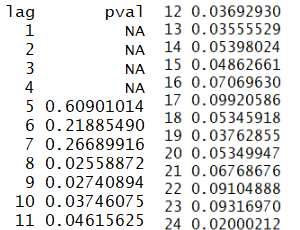
\includegraphics[scale =0.55]{qtest_aero.png}}
    \caption{Autocorrélation des résidus du modèle ARIMA(2,1,2)}
\end{figure}
\normalsize{
{L'absence d'autocorrélation des résidus est rejetée pour quasiment tous les lags pour le MA(1), mais seulement pour quelques-uns pour l'ARIMA(2,1,2). On sélectionne donc ce modèle faute de mieux, même s'il n'est pas parfaitement validé.
}}
\begin{tcolorbox}
{\small
5. Exprimer le modèle ARIMA(p,d,q) pour la série choisie.}
\end{tcolorbox}
\normalsize
{Nous avons sélectionné un $ARIMA(2, 1, 2)$, qui peut s'écrire :$X_t = -1.0811 X_{t-1} - 0.159 X_{t-2} + \varepsilon_t + 0.3543 \varepsilon_{t-1} - 0.5954\epsilon_{t-2}$
}\\ \\
\Large{\textbf{Partie III : Prévision}}
\begin{tcolorbox}
{\small
6. Ecrire l’équation vérifiée par la région de confiance de niveau \textbf{$\alpha$} sur les valeurs futures ($X_{T+1}, X_{T+2}$)}
\end{tcolorbox}
\normalsize
{En supposant les résidus gaussiens de même écart-type $\sigma$ ($\varepsilon_t \sim \mathcal{N}(0,\,\sigma^{2})$),  et en notant $q_{1- \alpha}$ le quantile d'ordre $1 - \alpha$ d'une ${\chi}^2(2)$ (2 étant le nombre de dimensions de la région de confiance), on a : \textbf{$R_{\alpha} = \lbrace x \in \mathbb{R}^2 | x^t \sigma x \leqslant q_{1-\alpha} \rbrace$ }}
\\
\begin{tcolorbox}
{\small
7. Préciser les hypothèses utilisées pour obtenir cette région.
}
\end{tcolorbox}
\normalsize{
{Nous avons besoin de deux hypothèses :
\begin{itemize}
\item Les coefficients estimés en Q4 et Q5 sont les coefficients théoriques de l'ARIMA ;
\item Les ($\varepsilon_t$) sont i.i.d., centrées et gaussiennes d'écart-type $\sigma^2$ positif connu.
\end{itemize}}}
\begin{tcolorbox}
{\small
8. Représenter graphiquement cette région pour $\alpha = 95$ \%. Commenter.
}
\end{tcolorbox}
\begin{figure}[h]
    \centering
    \fbox{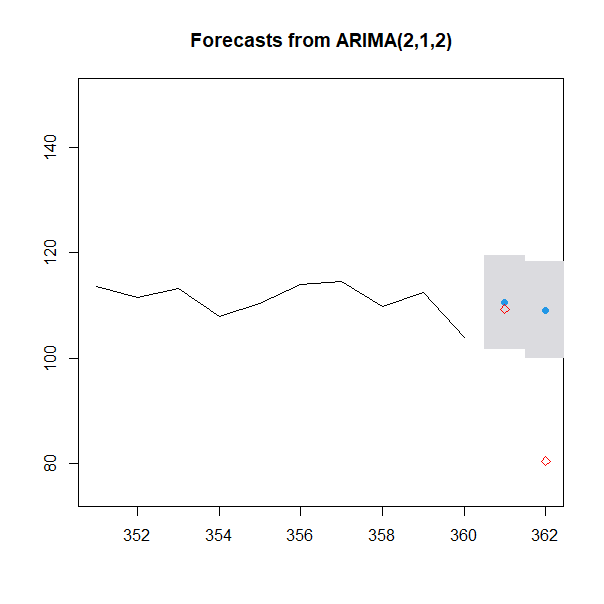
\includegraphics[scale =0.4]{predictions_212.png}}
    \caption{Prédictions pour les mois de février et mars 2020. Les points bleus représentent les valeurs prédites, la zone grise représente la région de confiance et les losanges représentent les valeurs réelles.}
\end{figure}
\normalsize{
{On représente ici les valeurs ($X_{T+1}, X_{T+2}$) (T=janvier 2020) avec leur région de confiance à 95 \%. La valeur prédite pour février 2020 est dans la région et est très proche de la valeur réelle, mais la valeur prédite pour mars 2020 n'est pas inclue dans la région de confiance. Cela s'explique par la forte baisse d'activité dans ce secteur conséquemment à la pandémie de COVID-19.\\
}}
\begin{tcolorbox}
{\small
9. Question ouverte : soit $Y_t$ une série stationnaire disponible de $t = 1$ à $T$. On suppose que $Y_{T+1}$
est disponible plus rapidement que $X_{T+1}$. Sous quelle(s) condition(s) cette information permet-elle
d’améliorer la prévision de $X_{T+1}$ ? Comment la (les) testeriez-vous ?
}
\end{tcolorbox}

\normalsize{
{$Y_{T+1}$ est utile dans la prédiction instantanée de $X_{T+1}$ ssi $Y$ cause $X$ instantanément au sens de Granger, soit : $\hat{X}_{T+1} | \lbrace Y_u, X_u, u < T \rbrace \cup \lbrace Y_{T+1} \rbrace \neq \hat{X}_{T+1} | \lbrace Y_u, X_u, u < T \rbrace$.\\
Afin de tester cette condition, (chapitre 5).
}}
\end{document}